\documentclass{layout/tudelft-report}

% Bibliography Sources
\addbibresource{bibliography/references.bib}
\addbibresource{bibliography/additional_references.bib}

% Define Notation commands
% Underlined vectors:
\def\x{\underline{x}}
\def\u{\underline{u}}
\def\p{\underline{p}}
\def\v{\underline{v}}
\def\q{\underline{q}}

% Control surface deflections
\def\del{\delta_{e}}
\def\dail{\delta_{a}}
\def\drud{\delta_{r}}

% Cal symbols
\def\H{{\cal H}}
\def\B{{\cal B}}
\def\D{{\cal D}}
\def\I{{\cal I}}
\def\N{{\cal N}}
\def\O{{\cal O}}
\def\U{{\cal U}}
\def\A{{\cal A}}
\def\S{{\cal S}}
\def\X{{\cal X}}
\def\R{{\cal R}}
\def\Z{{\cal Z}}
\def\P{{\cal P}}
\def\M{{\cal M}}
\def\L{{\cal L}}
\def\T{{\cal T}}

% Mathbb characters
\def\TT{{\mathbb{T}}}

% Parameter vectors
\def\k{{k}}
\def\w{{w}}

% Greek symbol shorthands
\def\eps{{\epsilon}}
\def\th{{\theta}}

\def\simc{\!\sim\!}
\def\ind#1{{\mathbbm 1}_{#1}}
\def\la{($\lambda$)\xspace}
\def\vpi{v_\pi}
\def\vstar{v_*}
\def\qpi{q_\pi}
\def\qstar{q_*}

% || || 
\renewcommand{\norm}[1]{\left\Vert#1\right\Vert}

% || ||_p
\newcommand{\Lpnorm}[1]{\left\Vert#1\right\Vert_{p}}

% | |
\renewcommand{\abs}[1]{\left| #1 \right|}

% :=
\newcommand{\bydef}{\coloneqq}

% Curlies { . }
\newcommand{\curlies}[1]{\left\{ #1 \right\}}

% Set { . }
\newcommand{\set}[1]{\left\{ #1 \right\}}

% Square brackets [ . ]
\newcommand{\sqBrackets}[1]{\left[ #1 \right]}

% Tuple < . >
\newcommand{\tuple}[1]{\left\langle #1 \right\rangle}



% Equal by distributions:
\newcommand{\distrequal}{\overset{\mathcal{D}}{=}}

% Equal by distributions by definition:
\newcommand{\distrbydef}{\overset{\mathcal{D}}{\coloneqq}}

% Probability:
\renewcommand{\Pr}[2][]{
    \mathbb{P}_{#1}\sqBrackets{#2}
}

% Expectation:
\newcommand{\E}[2][]{
    \mathbb{E}_{#1}\sqBrackets{#2}
}

% Gradient:
\def\gradient{\nabla}

% Real numbers:
\def\Real{\mathbb{R}}

% Transpose:
\def\Tr{^\top}

% Nicer conditional:
\def\Vertical{~\vert~}

% argmax
\newcommand{\argmax}[2]{
    \underset{#1}{argmax}\left( #2 \right)
}

% log
\renewcommand{\log}[1]{\textsf{log}~#1}

% Theorems and stuff
\newtheorem{theorem}{Theorem}[section]

% Degrees
\renewcommand{\deg}{\si{\degree}\xspace}

% Short-hand commands
\def\HINF{{$H_{\infty}~$}}

\def\QLAMBDA{{$Q(\lambda$)-learning}}

\renewcommand{\max}[1]{
    \underset{#1}{\text{max}}~
}

\renewcommand{\argmax}[1]{
    \underset{#1}{\text{argmax}}~
}

\newcommand{\epsgreedy}[1]{
    \epsilon\text{-}greedy\left( #1 \right)
}

\newcommand{\clip}[1]{
    \text{clip}\left(#1\right)
}

% \num command to pretty print 1e-5
\def\num#1{\numx#1}\def\numx#1e#2{{#1}\mathrm{e}{#2}}


% Nomenclature
\makenomenclature

\begin{document}

    \frontmatter

    % Thesis Parameters
    \title{Thesis template}
    \subtitle{Subtitle to the thesis}
    \author{Author Name}
    \subject{Thesis Report}

    % Cover Page
    \makecover
    \afterpage{\blankpage}
    
    % Title Page
    \begin{titlepage}

\begin{center}

%% Print the title
{\makeatletter
\largetitlestyle\fontsize{45}{45}\selectfont\@title
\makeatother}

\bigskip

%% Print the subtitle
{\makeatletter
\vspace{12mm}
\ifdefvoid{\@subtitle}{}{\largetitlestyle\fontsize{20}{20}\selectfont\@subtitle}
\makeatother}

\bigskip
\bigskip

Thesis report

\bigskip
\bigskip

by

\bigskip
\bigskip

%% Print the name of the author
{\makeatletter
\largetitlestyle\fontsize{25}{25}\selectfont\@author
\makeatother}

\bigskip
\bigskip

to obtain the degree of Master of Science \\
at the Delft University of Technology \\
to be defended publicly on January 1, 1970 at 00:00

\vfill

%% Print some more information at the bottom
\begin{tabular}{ll}
\textit{Thesis committee}:      & \\
Chair:                          & Dr. XXX \\ 
Supervisors:                    & Dr. XXX \\
                                & XXX \\
External examiner:              & Dr. XXX \\ 
Place:                          & Faculty of Aerospace Engineering, Delft \\
Project Duration: & January, 1970 - January, 1970 \\
Student number: & XXXXXXX
\end{tabular}

\vspace*{1cm}

An electronic version of this thesis is available at \url{http://repository.tudelft.nl/}.

\vspace*{2cm}
  \begin{center}
    \begin{tabular}{lcr}
      Faculty of Aerospace Engineering & $\cdot$ & Delft University of Technology
    \end{tabular}
  \end{center}

\end{center}

\end{titlepage}

    
    % Copyright Page
    \begin{flushleft}
  \vspace*{15cm}
  \vspace*{\stretch{3}}
  \thispagestyle{empty}
  \noindent%
  
\includegraphics[width=55mm]{layout/tudelft/logo.png}\\  
  Copyright \copyright\ Author Name here, 2022 \\
  All rights reserved.
\end{flushleft}

    % Make a preface page
    \chapter*{Preface}

<preface>
    
    % TOC, Nomenclature, List of stuff
    \tableofcontents    
    \printnomenclature
    \listoffigures
    \listoftables

    %% Report
    \mainmatter
    % Abbreviations
\nomenclature[A]{ADP}{Approximate Dynamic Programming}
\nomenclature[A]{AI}{Artificial Intelligence}
\nomenclature[A]{ANN}{Artificial Neural Network}
\nomenclature[A]{CNN}{Convolutional Neural Network}
\nomenclature[A]{CPW}{Cumulative Probability Weighting}
\nomenclature[A]{DNN}{Deep Neural Network}
\nomenclature[A]{DOF}{Degree of freedom}
\nomenclature[A]{DP}{Dynamic Programming}
\nomenclature[A]{DPG}{Deterministic Policy Gradient}
\nomenclature[A]{DRL}{Deep Reinforcement Learning}
\nomenclature[A]{EOM}{Equations of Motion}
\nomenclature[A]{FCSD}{Flight Control System Design}
\nomenclature[A]{GPI}{Generalized Policy Iteration}
\nomenclature[A]{INDI}{Incremental Nonlinear Dynamic Inversion}
\nomenclature[A]{IID}{Independent and identically distributed}
\nomenclature[A]{LOC}{Loss of Control}
\nomenclature[A]{LQR}{Linear Quadratic Regulator}
\nomenclature[A]{MC}{Monte Carlo}
\nomenclature[A]{ML}{Machine Learning}
\nomenclature[A]{MSE}{Mean Squared Error}
\nomenclature[A]{nMAE}{Normalized Mean Absolute Error}
\nomenclature[A]{OBM}{On-board Model}
\nomenclature[A]{PID}{Proportional-Integral-Derivative}
\nomenclature[A]{RL}{Reinforcement Learning}
\nomenclature[A]{RMSE}{Root Mean Square Error}
\nomenclature[A]{RNN}{Recurrent Neural Network}
\nomenclature[A]{RQ}{Research Question}
\nomenclature[A]{SGD}{Stochastic Gradient Descent}
\nomenclature[A]{UAS}{Unmanned Aerial System}
\nomenclature[A]{UAV}{Unmanned Aerial Vehicle}
\nomenclature[A]{VTOL}{Vertical Take-off and Landing}
\nomenclature[A]{RV}{Random Variable}

% Greek letters
\nomenclature[S]{$ \delta $}{TD-error}
\nomenclature[S]{$ \eps $}{Exploration coefficient}
\nomenclature[S]{$ \eta $}{Entropy Temperature}
\nomenclature[S]{$ \kappa $}{Huber-loss parameter}
\nomenclature[S]{$ \xi $}{Risk-distortion parameter}
\nomenclature[S]{$ \Psi $}{Distortion risk-measure}
\nomenclature[S]{$ t $}{Time-step}

% Aerospace stuff
\nomenclature[S]{$ \underline{\delta} $}{Control surface deflections}
\nomenclature[S]{$ \del $}{Elevator deflection}
\nomenclature[S]{$ \dail $}{Aileron deflection}
\nomenclature[S]{$ \drud $}{Rudder deflection}
\nomenclature[S]{$ \phi $}{Roll angle}
\nomenclature[S]{$ \psi $}{Yaw angle}
\nomenclature[S]{$ \Omega $}{Angular velocity}
\nomenclature[S]{$ u $}{Forward velocity component}
\nomenclature[S]{$ v $}{Sideways velocity component}
\nomenclature[S]{$ w $}{Vertical velocity component}
\nomenclature[S]{$ q $}{Pitch rate}
\nomenclature[S]{$ \x $}{Dynamic state vector}
\nomenclature[S]{$ \u $}{Control input vector}
\nomenclature[S]{$ \alpha $}{Angle of attack}
\nomenclature[S]{$ \beta $}{Angle of sideslip}

    \chapter{Introduction}
\label{chapter:intro}

\section{Template description}

This template is made for thesis reports that require a scientific article to be part of the deliverable.
Create a standalone scientific article as a \texttt{PDF} and include it as Chapter 2.

The file \texttt{notation.tex} defines notation macros that are common in your thesis. For example, the expectation operator using \texttt{\textbackslash E}:

\begin{equation}
\E[\pi]{\sum_{t}^{\infty} \x_t}
\end{equation}

The file \texttt{styling.tex} defines official TU Delft colors, and uses primary, secondary and accent definitions to keep the color scheme consistent.
It also defines \texttt{tikz} styles for each shaded and non-shaded blocks for illustration.

Use XeLatex/LuaLatex to compile.

\section{Examples}

Here are a few example citations, for example the PDF: \cite{einstein1905electrodynamics}. Also \cite{mnih2015human}.

A figure with inserted \texttt{PNG} is shown in \cref{fig:example}.
In order to make nice tables, use booktabs and avoid vertical lines, as shown in \cref{tab:example}.
Add illustrations using tikz as shown in \cref{fig:fig_tikz}.

\begin{figure}[ht]
    \centering
    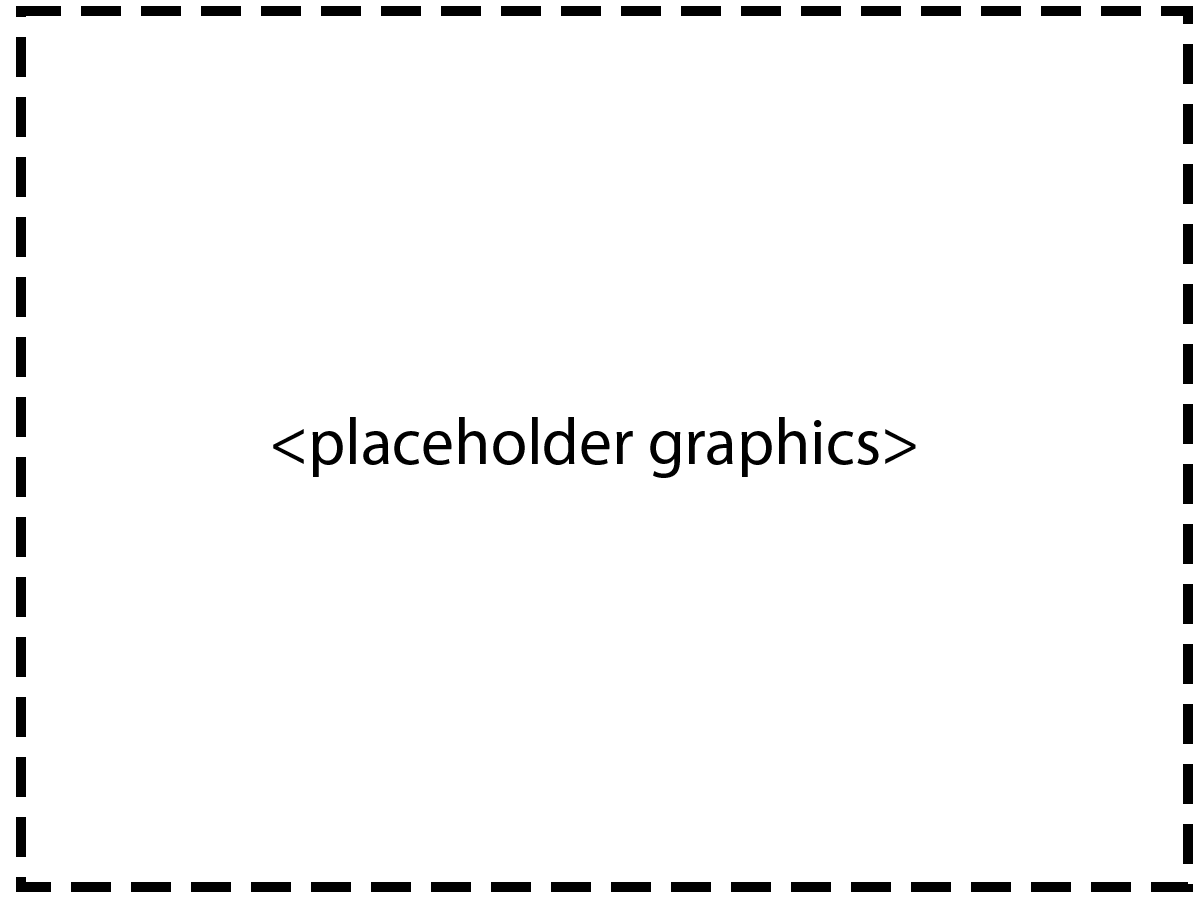
\includegraphics[width=0.4\textwidth]{figures/placeholder_black.png}
    \caption{This is an example figure}
    \label{fig:example}
\end{figure}

\begin{table}[ht]
    \centering
    \caption{Example clean table}
    \label{tab:example}
    \begin{tabular}{@{}ccc@{}}
    \toprule
    Altitude & $1,000 (m)$ & $2,000 (m)$ \\
    \midrule
    P &  0.2  & 0.4  \\ 
    I &  0.01 & 0.02 \\
    D &  0.4  & 0.5  \\
    \bottomrule
    \end{tabular}
\end{table}

\begin{figure}[ht]
    \centering
    \begin{tikzpicture}
        \node[block-primary] (ac) at (0, 0) {Aircraft};
        \node[shaded-primary] (co) at (-6, 0) {Controller};

        \draw[line] (co) -- node [midway, above] {u} (ac);
        \draw[line] (ac) to++ (0, -2) -| node [pos=0.25, below] {x} (co);
        
    \end{tikzpicture}
    \caption{This is an example tikz illustration.}
    \label{fig:fig_tikz}
\end{figure}

\newpage
\section{Research Formulation}
\label{section:intro-reseach-questions}

A few macros are defined to show the research questions and research objective in a box:

\ResearchObjective{The primary objective of this research project is to graduate.}

\ResearchQuestion{1}{What state-of-the-art methods are most suitable for XXX ?}

You can refer to your research question as: RQ \ref{rq:1}, which should generate a hyperlink.

\section{Structure of the Report}
\label{section:intro-report-structure}

% Scope
The purpose of this report is to (...)

% Structure of the paper
The structure of the report is as follows.
Firstly, \cref{chapter:article} shows Einstein's 1905 paper about special relativity as an example inserted standalone article pdf, in \cref{part:article}.
Then,(...)

    % Parts can have epigraphs to add notes
    \epigraphhead[650]{}
    \part{Scientific Article}
    \label{part:article}

    % __ Insert afterpage if to start chapters on the right side for print version.
    % \afterpage{\blankpage}

    % Place the scientific article pdf in here
    \clearpage
    \thispagestyle{empty}
    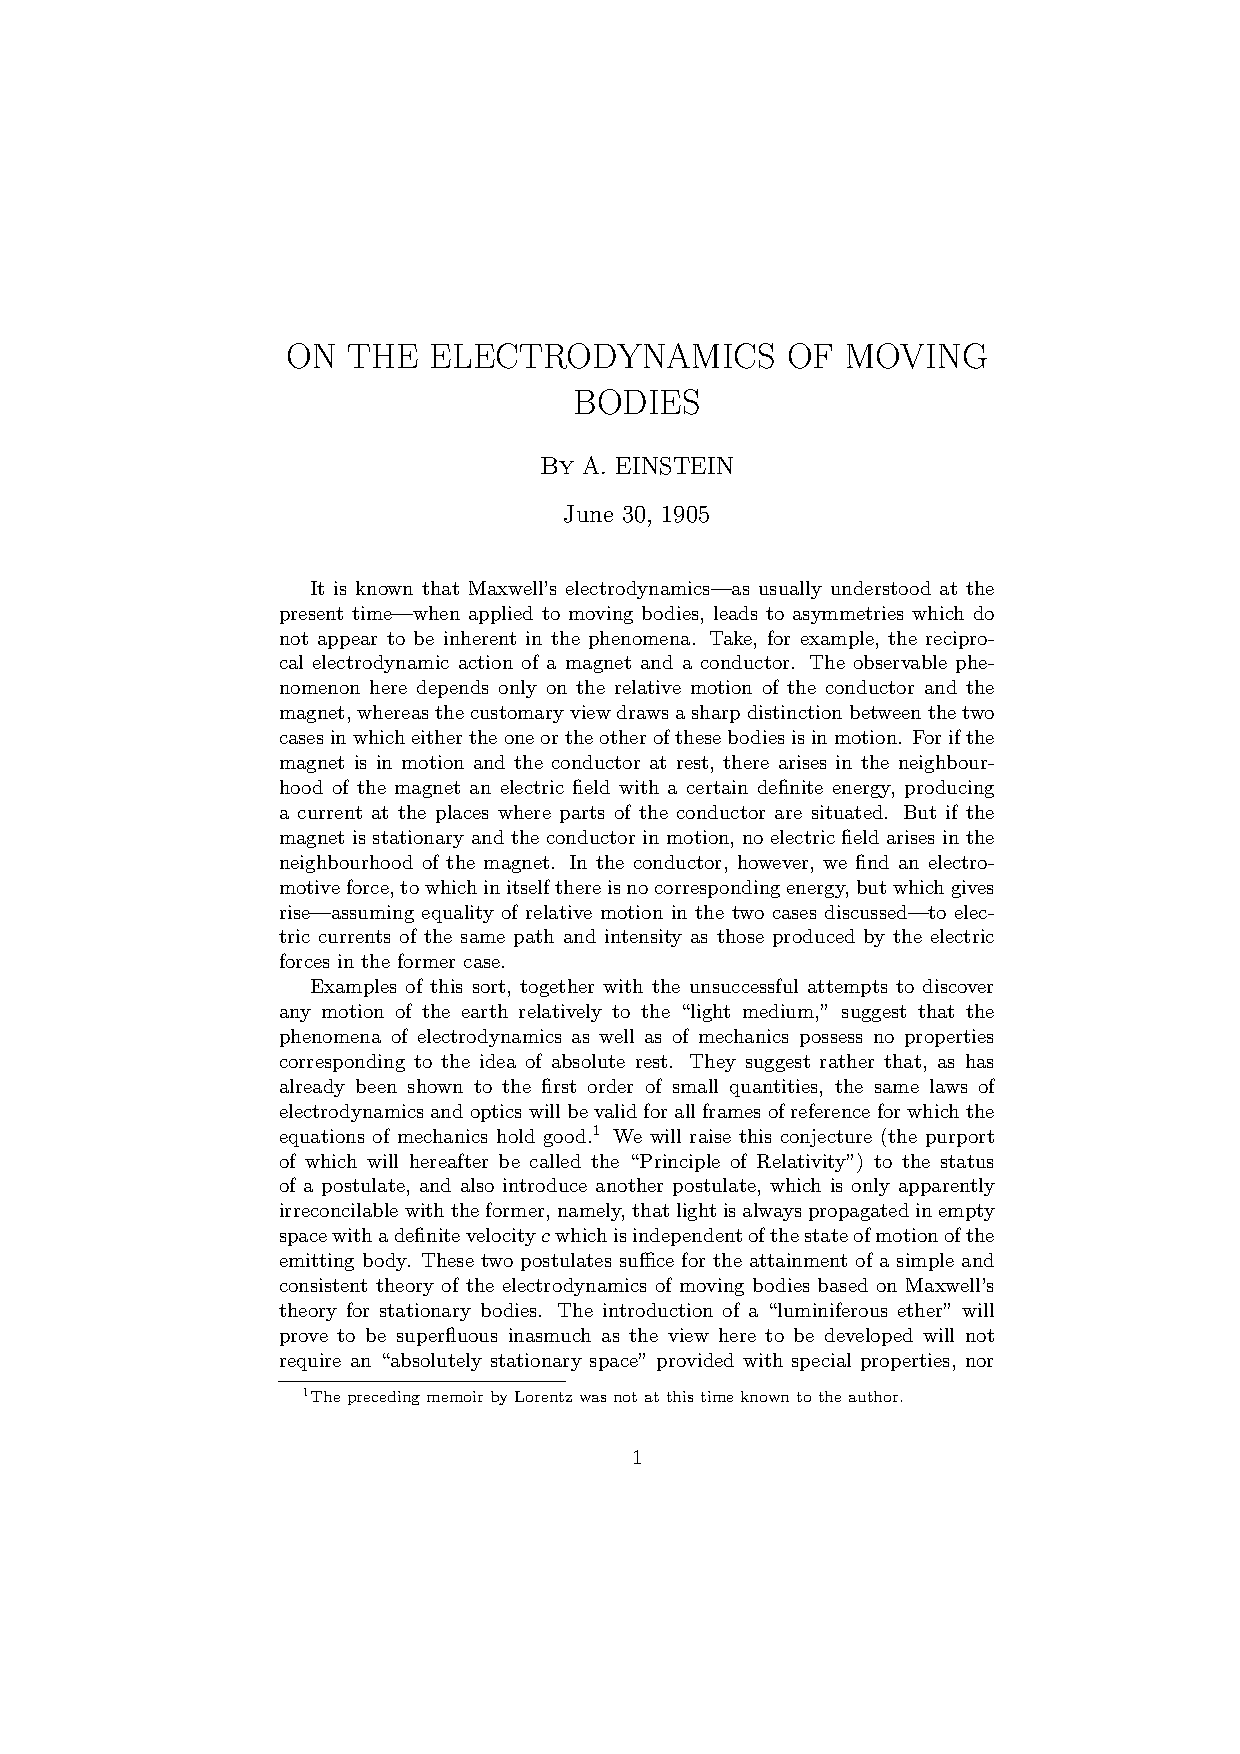
\includepdf[pages=-, addtotoc={
         1, chapter, 1, On the electrodynamics of moving bodies, chapter:article,
         1, section, 1, Introduction, section:articleintro,   
         2, section, 1, Background, section:articlebg,
         5, section, 1, Methodology, section:articlemethod,
         9, section, 1, Results \& Discussion, section:articleresults,
         11,section, 1, Conclusion, section:articleconc}
        ]{mainmatter/chapter-2-scientific-article.pdf}
    
    \newpage

    \epigraphhead[650]{*This part has been assessed for the course AE4020 Literature Study.}
    \part{Preliminary Analysis}
    \label{part:prelim}
    
    \chapter{Literature Review}
\label{chapter:lit_review}

% Leveldown and levelup commands allow to re-use chapters from the literature review but with different section levels.

\newenvironment{leveldown}% Demote sectional commands
  {\let\chapter\section
   \let\section\subsection%
   \let\subsection\subsubsection%
   \let\subsubsection\paragraph%
  }{}
  
\newenvironment{levelup}% Promote sectional commands
  {\let\subparagraph\paragraph%
   \let\paragraph\subsubsection%
   \let\subsubsection\subsection%
   \let\subsection\section%
   \let\section\chapter
}{}

\begin{leveldown}

\chapter{Lit Review Chapter 1}

\newpage
\chapter{Lit Review Chapter 2}

\newpage
\chapter{Lit Review Chapter 3}

\newpage
\chapter{Lit Review Chapter 4}

\end{leveldown}

    \chapter{Preliminary Work}
\label{chapter:prw}

\section{Methodology}
\label{section:prw-methodology}

\subsection{Environments}
\label{subsection:prw-env}

\subsection{Algorithms used}
\label{subsection:prw-algorithms}

\subsection{Training \& Evaluation}
\label{subsection:prw-training-and-eval}

\section{Results}
\label{section:prw-results}

\subsection{Learning performance}
\label{subsection:prw-learning-performance}

\section{Synthesis}
\label{section:prw-synthesis}

% - What did we learn here?

% - Did we answer any of the research questions?

% - What's next?


    \epigraphhead[650]{}
    \part{Additional Results}
    \label{part:additional}
    
    \chapter{More Results}
\label{chapter:more_results}

stuff
    \chapter{Verification and Validation}
\label{chapter:vv}


    \epigraphhead[650]{}
    \part{Closure}
    \label{part:closure}

    \chapter{Conclusion}
\label{chapter:conc}

\section{Closing Remarks}
\label{section:conc-closing-remarks}

\section{Research Questions}
\label{section:conc-research-questions}

The research questions posed in \cref{chapter:intro} are repeated below for convenience.

\RestateResearchQuestion{1}{What state-of-the-art methods are most suitable for XXX?}

Reflect on research questions.
    \chapter{Recommendations}
\label{chapter:rec}

This chapter provides a brief overview of the primary recommendations for the future continuation of this research project.

\subsubsection*{Rec 1}

\subsubsection*{Rec 2}


    % Bibliography with numeric style
    \printbibliography[title=References]
    \addcontentsline{toc}{chapter}{References}
    
    % __ Appendix ___
    \appendix
    \chapter{Algorithms}
\label{appendix:algorithms}

This appendix contains an example algorithm.
\setlength{\textfloatsep}{6pt}

\newcommand{\hh}{\hspace*{3pt}}

\SetKwInput{KwInit}{Init}
\SetKwInput{KwHyper}{Hyperparameters}

\IncMargin{0.25em}
\begin{algorithm}[ht]
\DontPrintSemicolon
\caption{On-policy Monte-Carlo control}\label{alg:MC-control}

\KwInit{$\M = \tuple{\S, \A, \P, \R, \gamma}, Q(s, a)$}
\KwHyper{$K$}
\KwResult{$\pi(s)$}

\For{episode $k \leftarrow 1$ \KwTo $K$}{
    
    \hh
    
    \emph{sample $t \in [0, T]$ transitions during episode $k$ using policy $\pi$}\;
    
    $\TT_k \leftarrow \set{S_t, A_t, R_{t+1}, \cdots, R_{T}}_{\pi} \sim \M$\;
    
    \For{$\tuple{a, s} \in \TT_k$}{
        $N(s, a) \leftarrow N(s, a) + 1$\;
        $Q(s, a) \leftarrow Q(s, a) + \frac{1}{N(s, a)} \left( G_t - Q(s, a) \right)$\;
    }

    \hh
    
    \emph{improve policy using updated action-value function}\;
    $\epsilon \leftarrow \frac{1}{k}$\;
    $\pi \leftarrow \epsgreedy{q}$\;
}
\end{algorithm}

    
\end{document}
